\subsection{Distribución radial de a pares}

La distribución radial de a pares, introducida en la sección \ref{s:observables},
puede ser utilizada para describir la estructura de materiales amorfos. Para el 
caso de sistemas que están conformados por más de un elemento se pueden analizar 
las distribuciones radiales de a pares parciales ~\cite{lamparter1995}, donde la 
$g_{ij}(r)$ representa la RDF de los átomos $j$ a una distancia $r$ alrededor de 
los átomos centrales $i$, y que es lo mismo que considerar $g_{ji}(r)$. Las 
figuras \ref{fig:rdf-LiLi}, \ref{fig:rdf-SiSi}, \ref{fig:rdf-SiLi} muestran los
resultados obtenidos para las RDF de Li-Li, Si-Si y Si-Li, respectivamente. En
cada una de ellas se analizan los cambios en la estructura que se dan para los
distintos valores de $x$ en Li$_x$Si estudiados, las curvas se calculan sobre las
estructuras minimizadas de la HD.

\begin{figure}[h!]
    \centering
    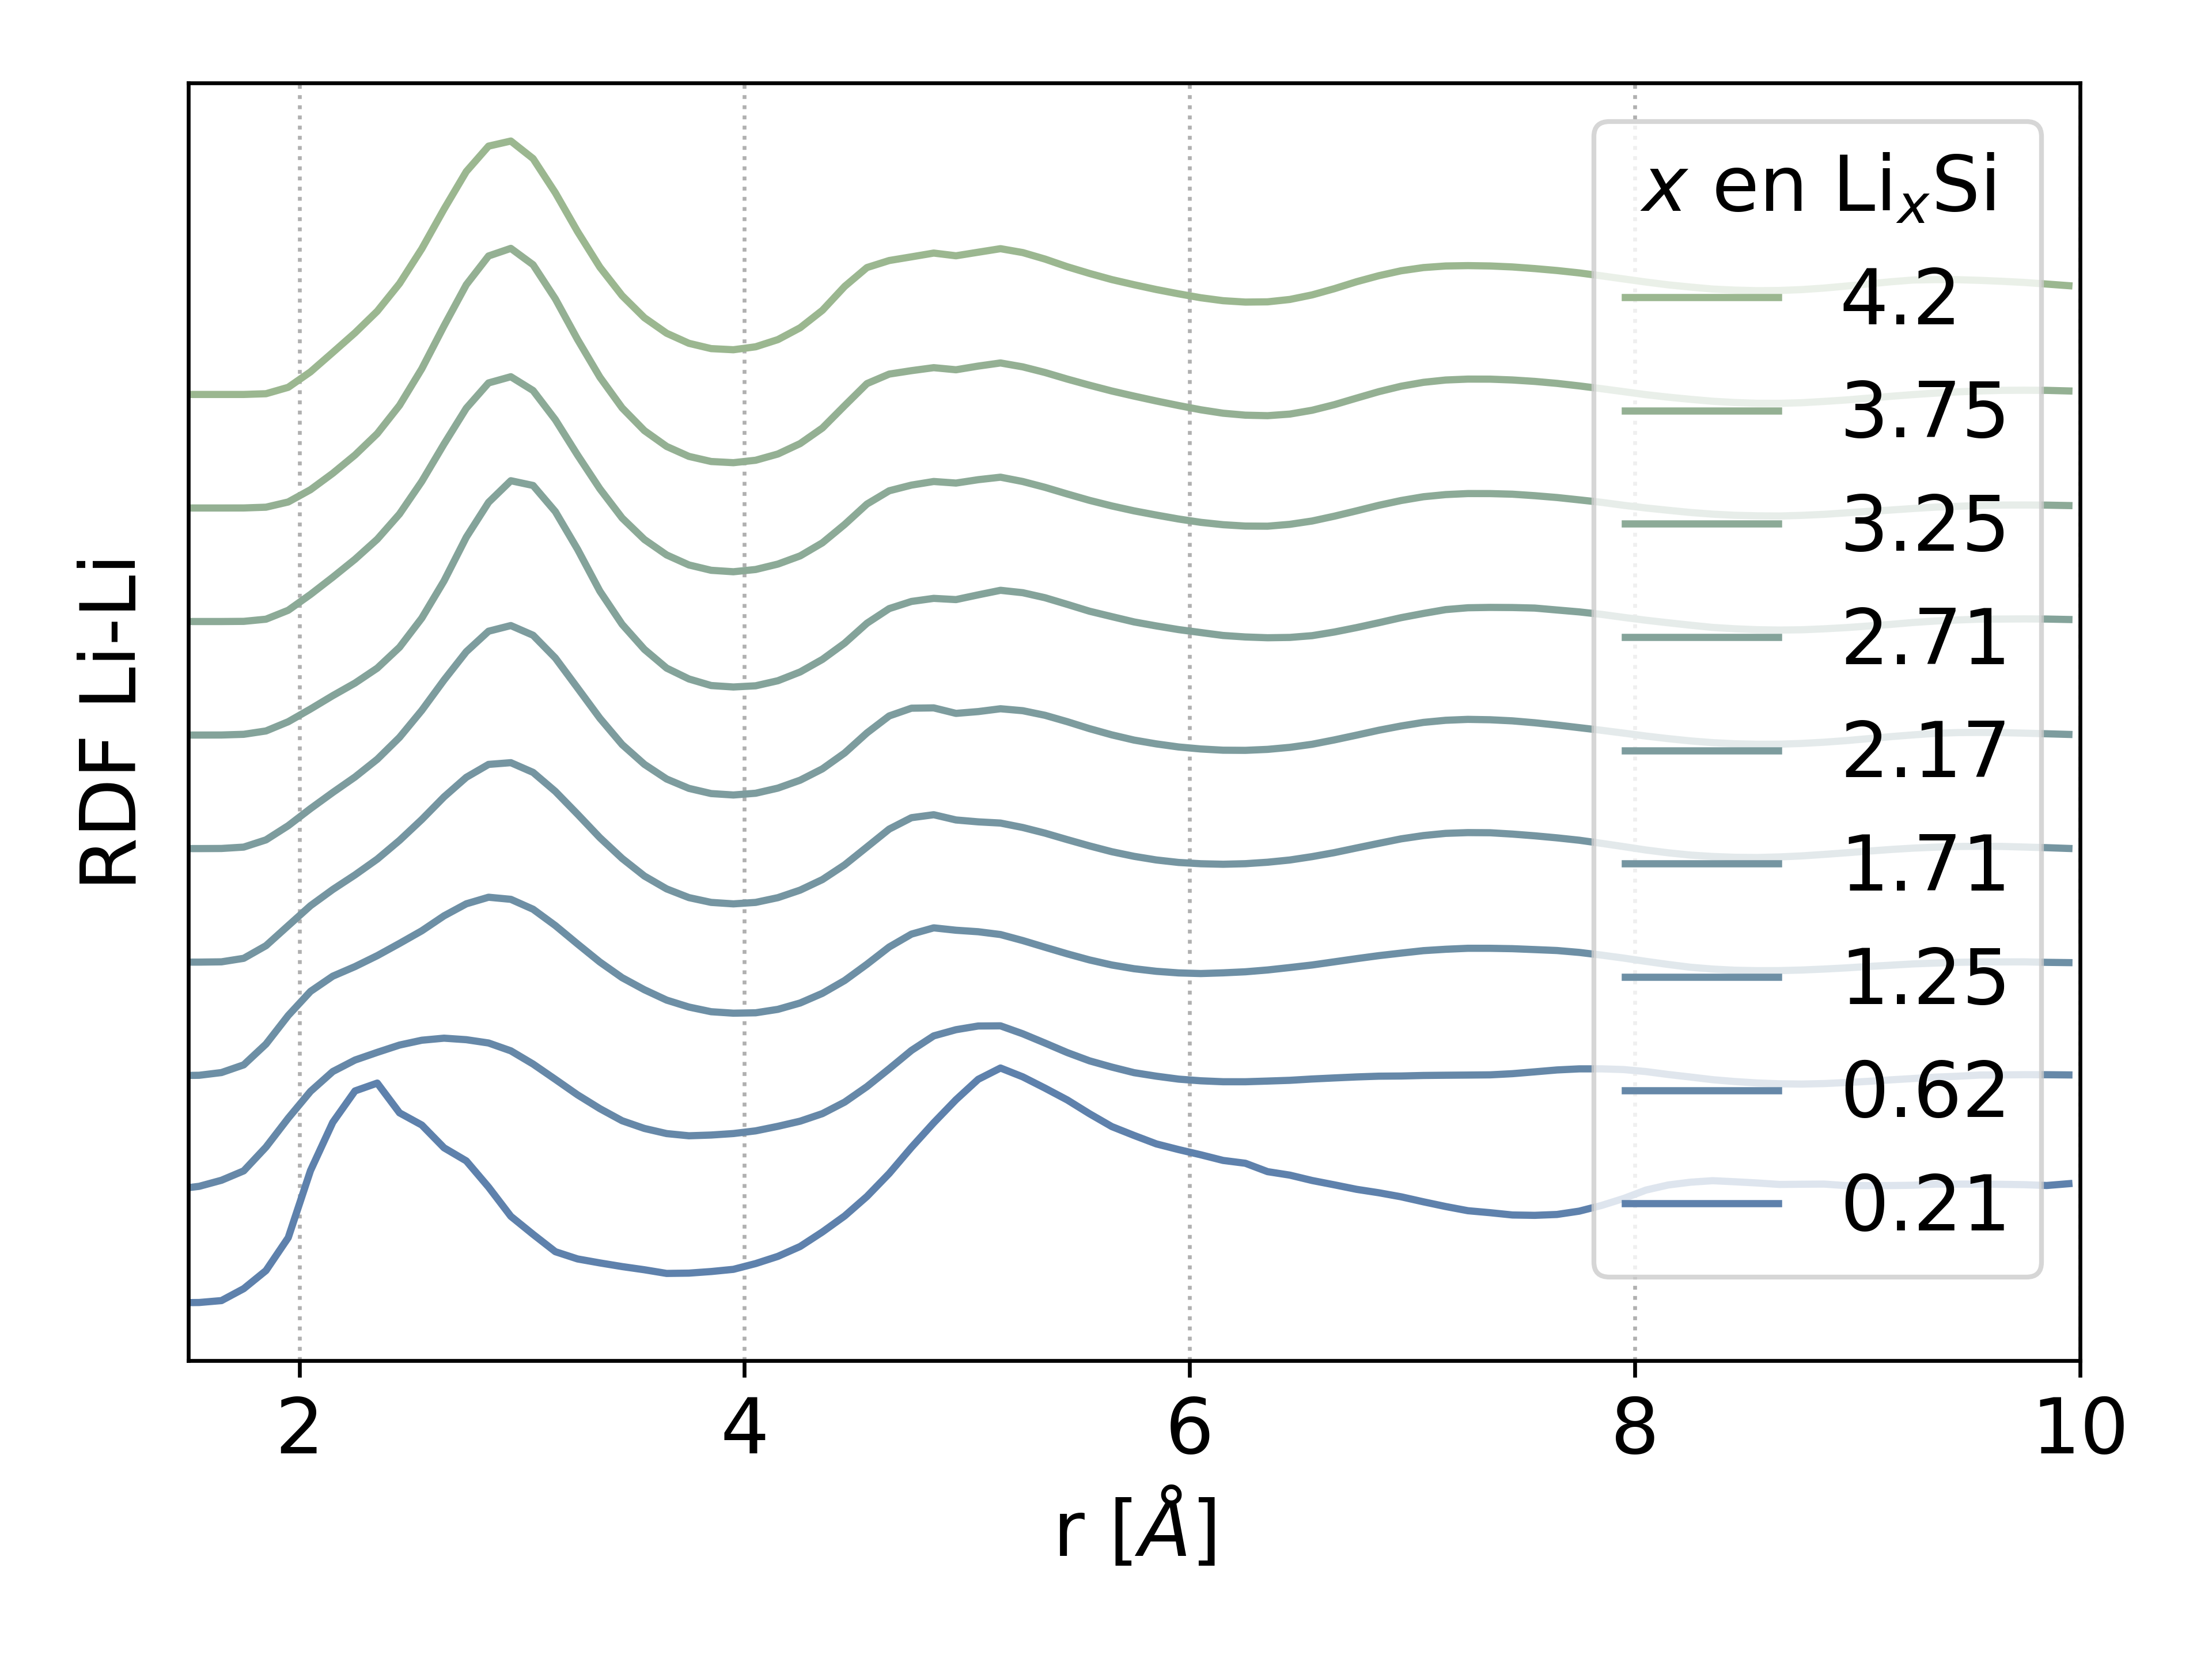
\includegraphics[width=0.8\textwidth]{caracterizacion/resultados/rdf/rdf-LiLi.png}
    \caption{Distribución radial de a pares para Li-Li de las estructuras 
    minimizadas. Cada curva se corresponde con un valor de concentración 
    distinto.}
    \label{fig:rdf-LiLi}
\end{figure}
Lo más relevante a destacar de la RDF$_{Li-Li}$ es que su primer pico comienza 
centrado en 2.45 \AA\ para las concentraciones de iones de Li más bajas y que 
luego dicho pico aumenta su posición a distancias más grandes a medida que aumenta
$x$ hasta permanecer en 2.95 \AA\ para $x$ mayores a 1.71. La altura de este pico
aumenta en un 50\% luego de la litiación completa, relativa a la menor 
concentración.

\begin{figure}[h!]
    \centering
    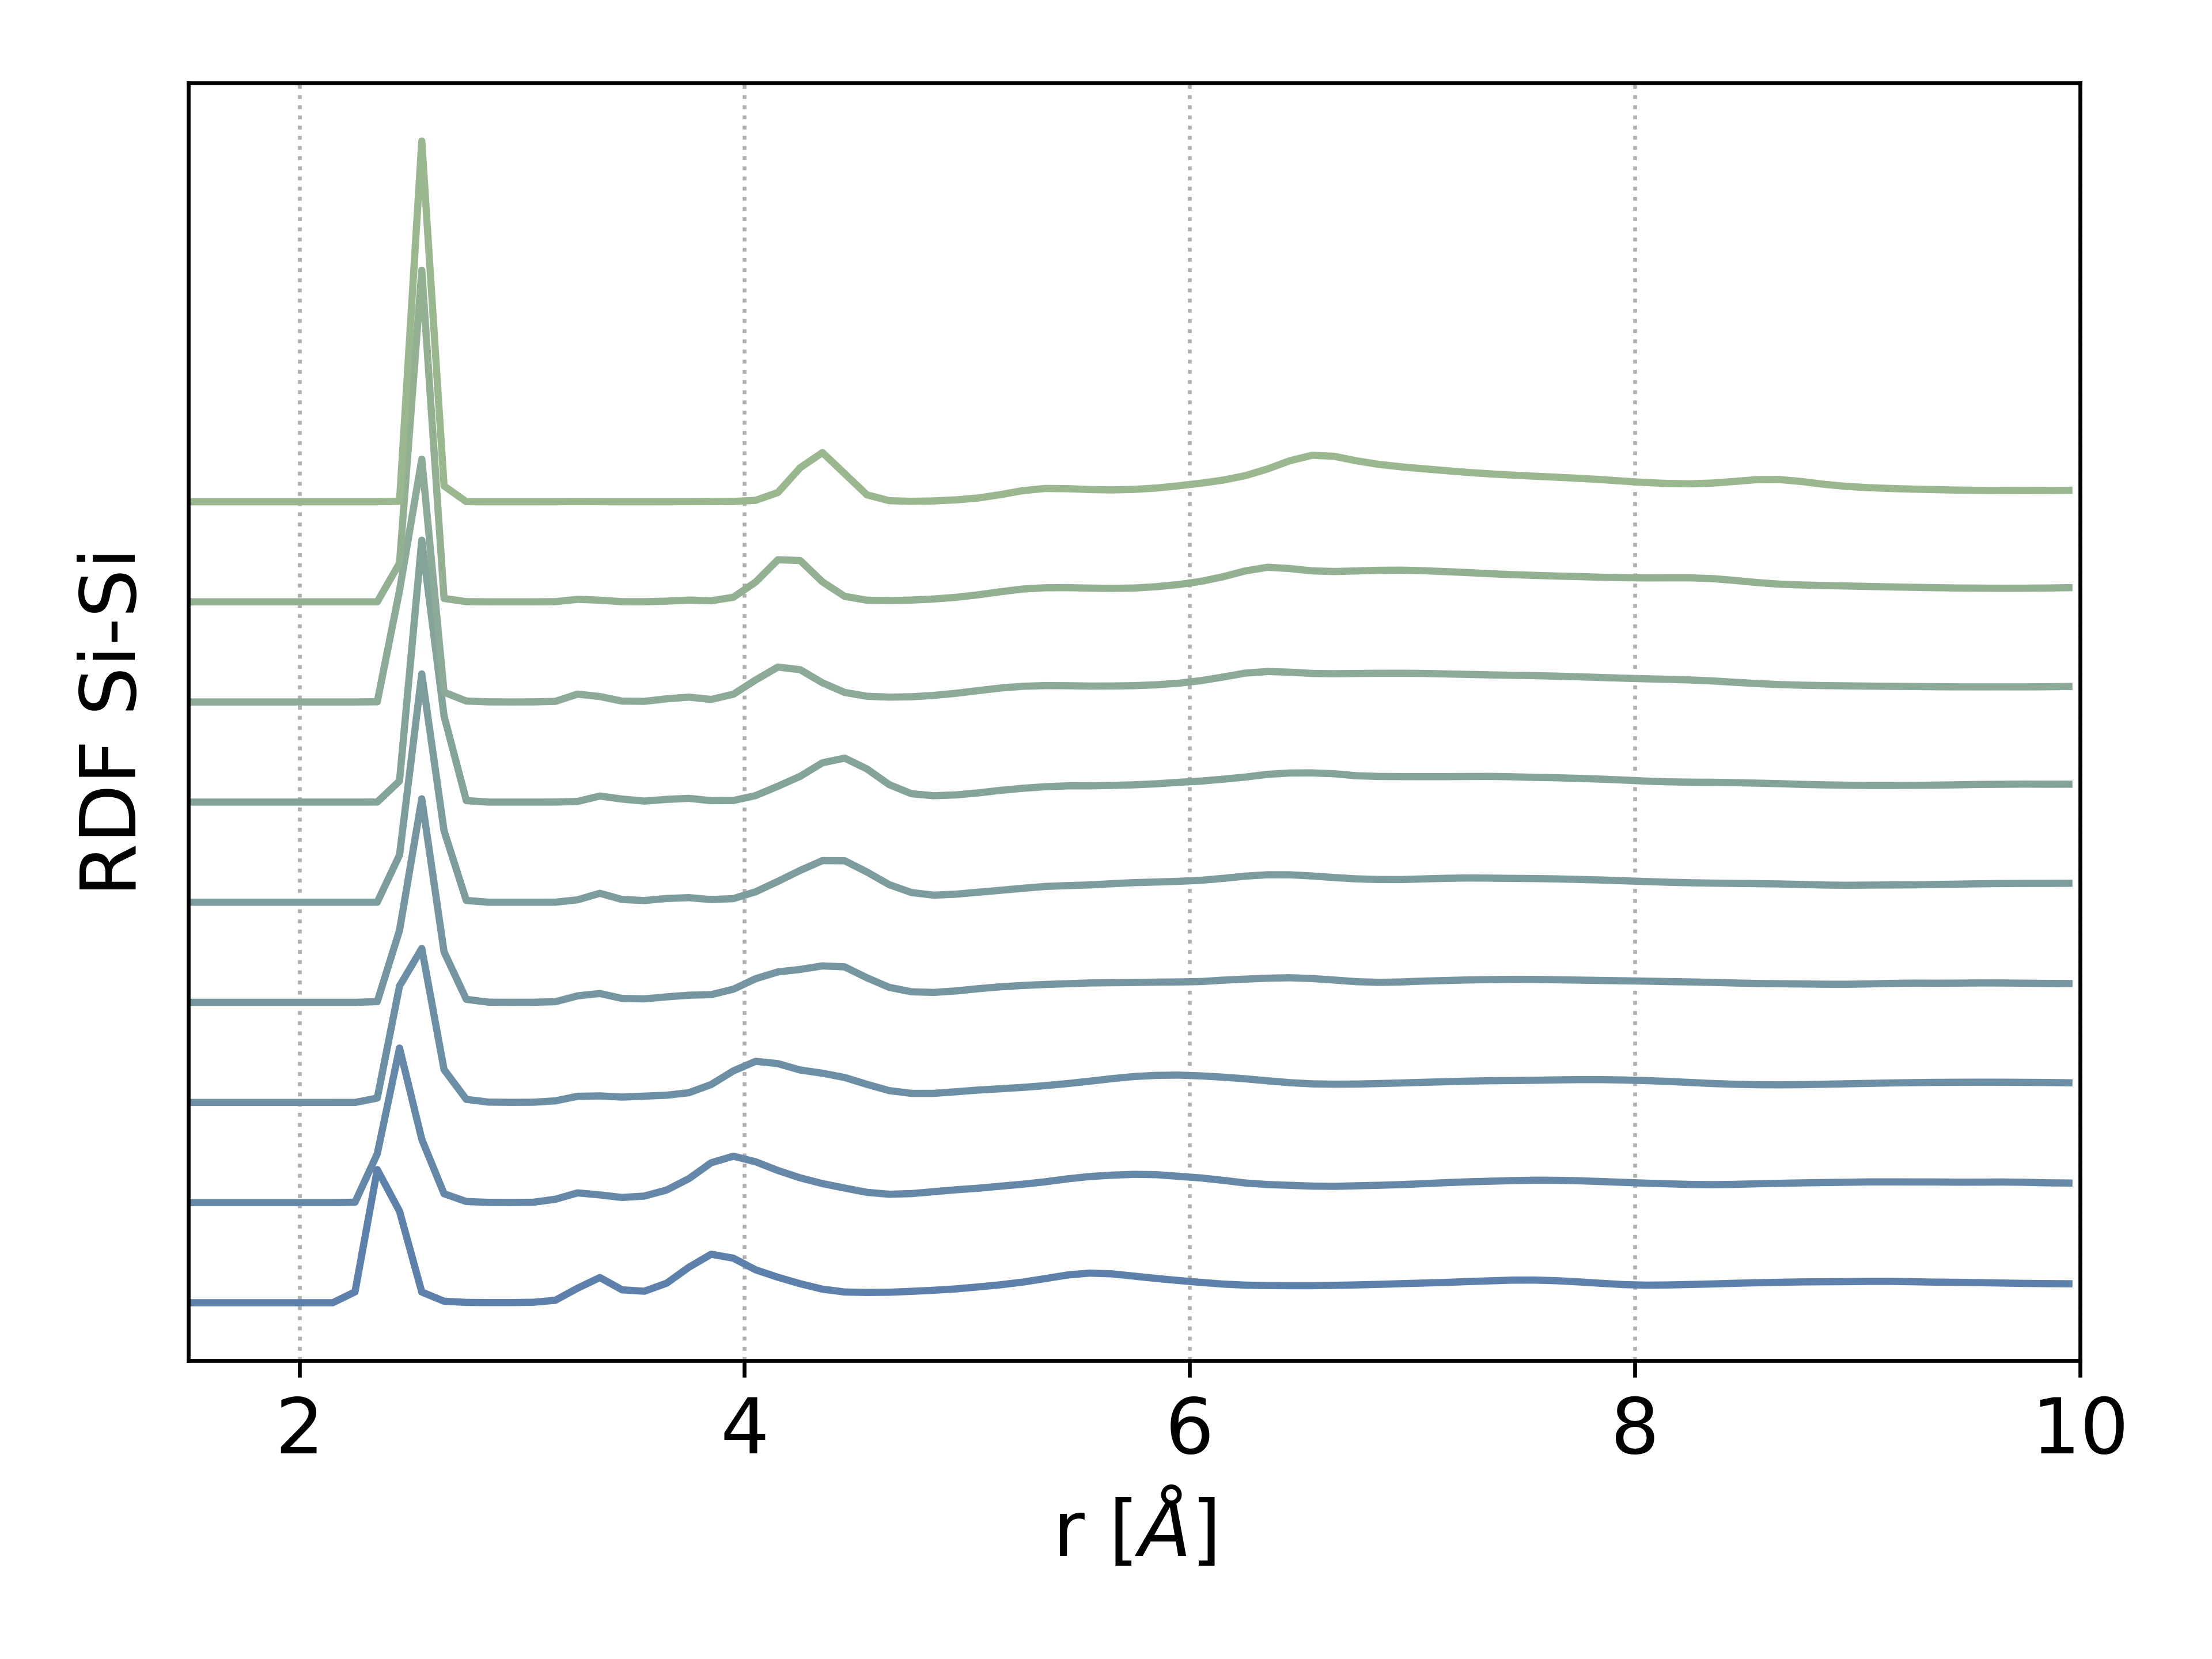
\includegraphics[width=0.8\textwidth]{caracterizacion/resultados/rdf/rdf-SiSi.png}
    \caption{Distribución radial de a pares para Si-Si de las estructuras 
    minimizadas. Cada curva se corresponde con un valor de concentración 
    distinto.}
    \label{fig:rdf-SiSi}
\end{figure}
Este mismo efecto se ve en el primer pico de la RDF$_{Si-Si}$, el centro del mismo
se encuentra en 2.4 \AA\ para $x = 0.21$ y luego se desplaza a distancias
mayores, después de $x = 1.25$ el centro se encuentra entre 2.52 y 2.56 \AA.
Mientras que la altura del pico aumenta se ve un decrecimiento en en el ancho 
del pico, el valor del FWHM va de 0.14 \AA\ a 0.05 \AA\ para $x = 0.21$ y 
$x = 3.75$, respectivamente. Por otro lado, el segundo pico de la RDF$_{Si-Si}$
también se desplaza hacia distancias mayores, se divide en dos picos para valores 
de $x$ entre 0.62 y 1.71 y vuelve a comportarse como un sólo pico para para 
concentraciones mayores. Entre el primer y el segundo pico se observa un hombro,
como señalaron previamente Fan \textit{et al.} ~\cite{fan2013}. Los resultados 
obtenidos para la RDF$_{Si-Si}$ están en concordancia con las mediciones 
experimentales reportadas por Key \textit{et al.} ~\cite{key2011}.

\begin{figure}[h!]
    \centering
    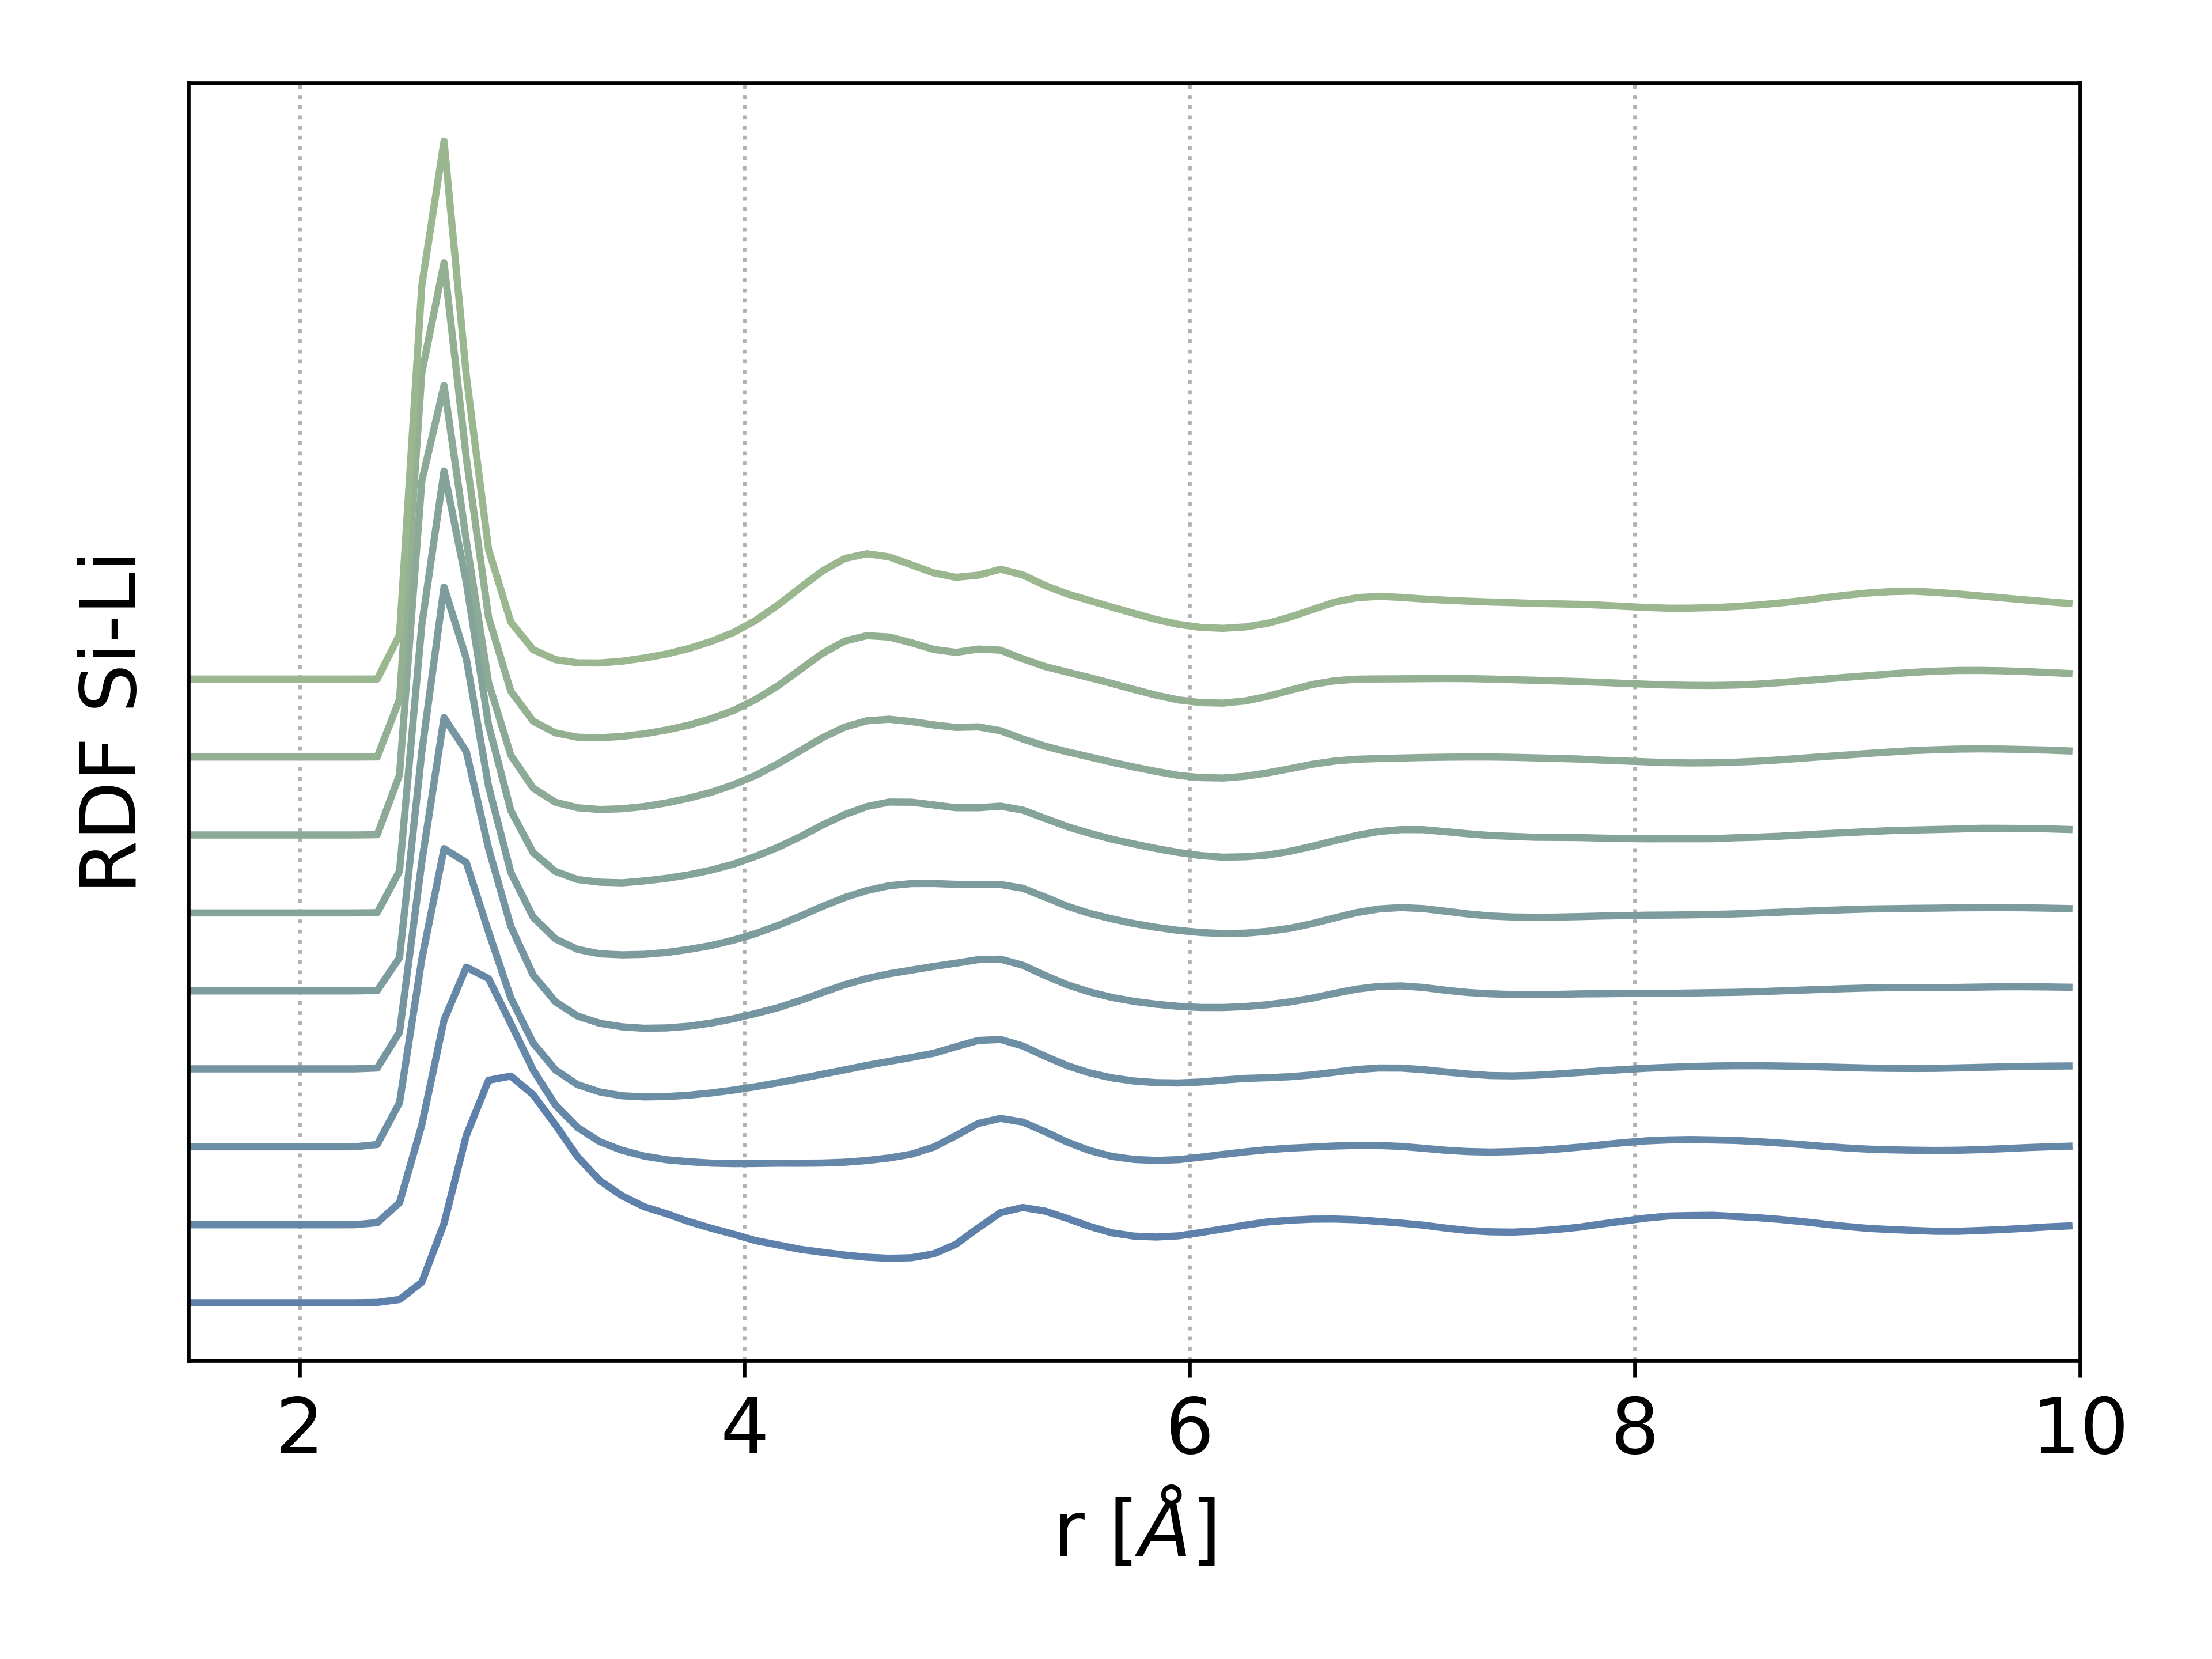
\includegraphics[width=0.8\textwidth]{caracterizacion/resultados/rdf/rdf-SiLi.png}
    \caption{Distribución radial de a pares para Si-Li de las estructuras 
    minimizadas. Cada curva se corresponde con un valor de concentración 
    distinto.}
    \label{fig:rdf-SiLi}
\end{figure}
Para el primer pico de la RDF$_{Si-Li}$ se ve el comportamiento contrario, el 
centro del mismo se desplaza a distancias menores a medida que la concentración
de litio aumenta. Esto es acompañado con un aumento de la altura del pico y una
disminución de su ancho. Para el segundo pico también se observa un desplazamiento
del mismo hacia distancias menores, pero por encima de $x = 1.71$ el pico se
divide en dos picos con distintas alturas dependiendo de la concentración. Esto
es analizado con mayor detalle en la sección \ref{s:intercionexion}.
